\documentclass[border=5pt]{standalone}
\usepackage[defaultfam,tabular,lining]{montserrat}
\usepackage[T1]{fontenc}
\renewcommand{\familydefault}{\sfdefault}
\usepackage[eulergreek]{sansmath}
\sansmath
\usepackage{tikz}
\usetikzlibrary{arrows.meta, positioning, calc}
\usepackage{fontawesome5}

% Palette
\definecolor{inkblack}{HTML}{111111}
\definecolor{pbpurple}{HTML}{6D28D9}
\definecolor{pbpurplefill}{HTML}{F5F3FF}
\definecolor{warnred}{HTML}{B91C1C}
\definecolor{warnredfill}{HTML}{FEF2F2}
\definecolor{devicegrey}{HTML}{94A3B8}
\definecolor{devicefill}{HTML}{E2E8F0}
\definecolor{trustteal}{HTML}{0D9488}
\definecolor{trusttealfill}{HTML}{F0FDFA}
\definecolor{dimgrey}{HTML}{C4B5FD}

\newcommand{\treeicon}[3]{%
  % #1,#2 = position, #3 = color
  \begin{scope}[shift={(#1,#2)}, scale=0.4]
    \fill[#3] (0,0) circle (3pt);
    \fill[#3] (-0.7,-0.55) circle (3pt);
    \fill[#3] (0.7,-0.55) circle (3pt);
    \fill[#3] (-1.05,-1.1) circle (2.5pt);
    \fill[#3] (-0.35,-1.1) circle (2.5pt);
    \fill[#3] (0.35,-1.1) circle (2.5pt);
    \fill[#3] (1.05,-1.1) circle (2.5pt);
    \draw[#3, line width=0.6pt] (0,0) -- (-0.7,-0.55);
    \draw[#3, line width=0.6pt] (0,0) -- (0.7,-0.55);
    \draw[#3, line width=0.5pt] (-0.7,-0.55) -- (-1.05,-1.1);
    \draw[#3, line width=0.5pt] (-0.7,-0.55) -- (-0.35,-1.1);
    \draw[#3, line width=0.5pt] (0.7,-0.55) -- (0.35,-1.1);
    \draw[#3, line width=0.5pt] (0.7,-0.55) -- (1.05,-1.1);
  \end{scope}%
}

\begin{document}
\begin{tikzpicture}[
    font=\footnotesize,
    cbox/.style 2 args={draw=#1, fill=#2, rounded corners=3pt, minimum height=1.5cm,
                        text width=2.5cm, align=center, line width=1.2pt, text=inkblack},
    inst/.style={cbox={warnred}{warnredfill}},
    aggA/.style={cbox={inkblack}{white}},
    aggB/.style={cbox={pbpurple}{pbpurplefill}},
    shB/.style={cbox={pbpurple}{pbpurplefill}},
    mbox/.style={draw=inkblack, fill=white, rounded corners=3pt,
                 minimum height=1.1cm, minimum width=1.4cm, align=center,
                 line width=1pt},
    clientbox/.style={draw=inkblack, fill=white, rounded corners=4pt, line width=1pt},
    arr/.style={-{Stealth[length=5pt,width=3.5pt]}, line width=1.1pt, inkblack},
    arrpb/.style={-{Stealth[length=5pt,width=3.5pt]}, line width=1.1pt, pbpurple},
    ret/.style={-{Stealth[length=5pt,width=3.5pt]}, line width=1.1pt, inkblack, densely dashed},
    retpb/.style={-{Stealth[length=5pt,width=3.5pt]}, line width=1.1pt, pbpurple, densely dashed},
    lbl/.style={font=\scriptsize\bfseries, text=inkblack, inner sep=2pt},
    lblret/.style={font=\scriptsize, text=inkblack, inner sep=2pt},
  ]

  % ===== PANEL A: Cross-Silo (bottom-to-top) =====
  \begin{scope}

    \node[font=\normalsize\bfseries, text=inkblack] at (3.0, 5.0) {(a) Cross-Silo Federated Learning};

    % --- Top tier: Aggregator + Model ---
    \node[aggA, minimum height=1.5cm, text width=2.8cm] (aggA) at (2.8, 3.6)
      {{\normalsize\faServer}\\[-1pt]\textbf{Aggregator}};
    \node[mbox] (modelA) at (7.2, 3.6) {};
    \treeicon{7.2}{3.85}{inkblack}
    \node[font=\tiny\bfseries, text=inkblack] at (7.2, 3.25) {Model};

    % --- Middle tier: Institutions ---
    \node[inst, text width=2.2cm] (iA) at (0,  1.3) {{\normalsize\faHospital}\\[-1pt]\textbf{Institution A}\\[1pt]{\tiny\itshape has access to all\\[-4pt]patient records}};
    \node[inst, text width=2.2cm] (iB) at (2.8, 1.3) {{\normalsize\faHospital}\\[-1pt]\textbf{Institution B}\\[1pt]{\tiny\itshape has access to all\\[-4pt]patient records}};
    \node[inst, text width=2.2cm] (iC) at (5.6, 1.3) {{\normalsize\faHospital}\\[-1pt]\textbf{Institution C}\\[1pt]{\tiny\itshape has access to all\\[-4pt]patient records}};

    % --- Bottom tier: Patient devices grouped per institution ---
    % Group A: 3 patients under Institution A
    \foreach \i in {0,...,2} {
      \pgfmathsetmacro{\xx}{-0.5 + \i*0.45}
      \draw[devicegrey, fill=devicefill, rounded corners=1.5pt, line width=0.5pt]
        (\xx, -1.02) rectangle ++(0.3, 0.44);
      \draw[devicegrey, fill=devicegrey, line width=0.3pt, rounded corners=0.5pt]
        (\xx+0.05, -0.66) rectangle ++(0.2, 0.04);
    }
    % Group B: 2 patients under Institution B
    \foreach \i in {0,...,1} {
      \pgfmathsetmacro{\xx}{2.35 + \i*0.45}
      \draw[devicegrey, fill=devicefill, rounded corners=1.5pt, line width=0.5pt]
        (\xx, -1.02) rectangle ++(0.3, 0.44);
      \draw[devicegrey, fill=devicegrey, line width=0.3pt, rounded corners=0.5pt]
        (\xx+0.05, -0.66) rectangle ++(0.2, 0.04);
    }
    % Group C: 4 patients under Institution C
    \foreach \i in {0,...,3} {
      \pgfmathsetmacro{\xx}{4.8 + \i*0.45}
      \draw[devicegrey, fill=devicefill, rounded corners=1.5pt, line width=0.5pt]
        (\xx, -1.02) rectangle ++(0.3, 0.44);
      \draw[devicegrey, fill=devicegrey, line width=0.3pt, rounded corners=0.5pt]
        (\xx+0.05, -0.66) rectangle ++(0.2, 0.04);
    }

    % Trust boundaries: each encloses one institution + its patient group
    \draw[warnred, densely dashed, line width=1.2pt, rounded corners=5pt, fill=warnredfill, fill opacity=0.3]
      (-1.3, -1.35) rectangle (1.3, 2.2);
    \draw[warnred, densely dashed, line width=1.2pt, rounded corners=5pt, fill=warnredfill, fill opacity=0.3]
      (1.5, -1.35) rectangle (4.1, 2.2);
    \draw[warnred, densely dashed, line width=1.2pt, rounded corners=5pt, fill=warnredfill, fill opacity=0.3]
      (4.3, -1.35) rectangle (6.9, 2.2);
    \node[font=\tiny\bfseries, text=warnred] at (0, -1.55) {trust boundary};

    % Arrows: patients -> institutions (vertical, raw data)
    \draw[arr] (0, -0.5) -- (iA.south);
    \draw[arr] (2.8, -0.5) -- (iB.south);
    \draw[arr] (5.6, -0.5) -- (iC.south);
    \node[lbl, text=warnred, anchor=east] at (0.0, 0.0) {raw data};

    % Arrows: institutions -> aggregator (upward, weights)
    \draw[arr] (iA.north) -- ([xshift=-10pt]aggA.south);
    \draw[arr] (iB.north) -- (aggA.south);
    \draw[arr] (iC.north) -- ([xshift=10pt]aggA.south);
    \node[lbl] at (-0.5, 2.55) {gradients};

    % Arrow: aggregator -> model
    \draw[arr] (aggA.east) -- (modelA.west);

    % Arrow: model -> institutions (return, dashed)
    \draw[ret] (modelA.south) -- (7.2, -0.8) -- (6.9, -0.8);

    % Caption
    \node[font=\scriptsize\bfseries\itshape, text=warnred] at (3.0, -2.1) {Institutions see raw patient data};
  \end{scope}

  % ===== PANEL B: PrivateBoost =====
  \begin{scope}[xshift=10.5cm]

    \node[font=\normalsize\bfseries, text=inkblack] at (3.2, 5.0) {(b) PrivateBoost};

    % Aggregator (top center)
    \node[aggB, text width=2.8cm] (aggB) at (2.8, 3.6)
      {{\normalsize\faServer}\\[-1pt]\textbf{Aggregator}};

    % Model (right of aggregator)
    \node[mbox] (modelB) at (7.2, 3.6) {};
    \treeicon{7.2}{3.85}{inkblack}
    \node[font=\tiny\bfseries, text=inkblack] at (7.2, 3.25) {Model};

    % Shareholders (middle row) with distinct icons
    \node[shB, text width=2.2cm] (sh1) at (0,  1.3) {{\normalsize\faHospital}\\[-1pt]\textbf{Shareholder 1}\\[-2pt]{\tiny\itshape e.g.\ Hospital}};
    \node[shB, text width=2.2cm] (sh2) at (2.8, 1.3) {{\normalsize\faCloud}\\[-1pt]\textbf{Shareholder 2}\\[-2pt]{\tiny\itshape e.g.\ Cloud}};
    \node[shB, text width=2.2cm, draw=dimgrey, text=devicegrey, fill=white] (sh3) at (5.6, 1.3) {{\normalsize\faLandmark}\\[-1pt]\textbf{Shareholder 3}\\[-2pt]{\tiny\itshape e.g.\ Regulator}};

    % Clients box (bottom)
    \node[clientbox, minimum width=7.6cm, minimum height=1.3cm] (clients) at (2.8, -0.8) {};

    % Device icons inside client box
    \foreach \i in {0,...,9} {
      \pgfmathsetmacro{\xx}{0.1 + \i*0.64}
      \draw[devicegrey, fill=devicefill, rounded corners=1.5pt, line width=0.5pt]
        (\xx, -1.02) rectangle ++(0.3, 0.44);
      \draw[devicegrey, fill=devicegrey, line width=0.3pt, rounded corners=0.5pt]
        (\xx+0.05, -0.66) rectangle ++(0.2, 0.04);
    }
    \node[font=\tiny\bfseries, text=inkblack] at (2.8, -1.25) {Clients (1 sample each)};

    % Trust boundaries around individual devices
    \foreach \i in {0,...,9} {
      \pgfmathsetmacro{\xx}{0.1 + \i*0.64}
      \draw[trustteal, densely dashed, line width=0.7pt, rounded corners=2pt]
        (\xx-0.08, -1.1) rectangle ++(0.46, 0.62);
    }
    \node[font=\tiny\bfseries, text=trustteal] at (2.8, -0.3) {trust boundary = each device};

    % Arrows: highlighted client -> all 3 shareholders
    \draw[arrpb] (0.25, -0.45) -- (sh1.south);
    \draw[arrpb] (0.25, -0.45) -- (sh2.south);
    \draw[-{Stealth[length=4pt,width=3pt]}, line width=1.1pt, dimgrey, densely dashed] (0.25, -0.45) -- (sh3.south);
    \node[lbl] at (-1.1, 0.35) {secret shares};

    % Arrows: shareholders -> aggregator
    \draw[arrpb] (sh1.north) -- ([xshift=-10pt]aggB.south);
    \draw[arrpb] (sh2.north) -- (aggB.south);
    \draw[-{Stealth[length=4pt,width=3pt]}, line width=1.1pt, dimgrey, densely dashed] (sh3.north) -- ([xshift=10pt]aggB.south);
    \node[lbl] at (-0.5, 2.55) {partial sums};
    % m-of-k threshold annotation
    \node[font=\tiny\bfseries\itshape, text=inkblack, anchor=west, align=left] at (4.6, 2.75) {threshold reconstruction\\($m$-of-$k$)};

    % Arrow: aggregator -> model
    \draw[arrpb] (aggB.east) -- (modelB.west);

    % Arrow: model -> clients (down far right, then left into clients)
    \draw[retpb] (modelB.south) -- (7.2, -0.8) -- (clients.east);

    % Caption
    \node[font=\scriptsize\bfseries\itshape, text=pbpurple] at (3.2, -2.1) {No party sees individual patient data};
  \end{scope}

\end{tikzpicture}
\end{document}
